% 2017 全国Ⅰ卷 理2/文4：正方形内的太极图（黑白关于中心成中心对称）
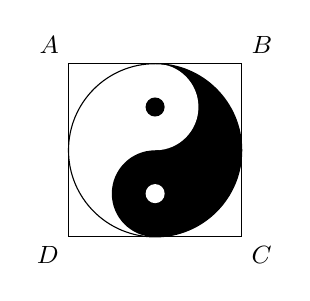
\begin{tikzpicture}[scale=1.1, font=\small]
  % 正方形 ABCD（A 左上、B 右上、C 右下、D 左下），边长 2，内切圆半径 1
  \draw (-1,-1) rectangle (1,1);
  \node[above left]  at (-1, 1) {$A$};
  \node[above right] at ( 1, 1) {$B$};
  \node[below right] at ( 1,-1) {$C$};
  \node[below left]  at (-1,-1) {$D$};
  \begin{scope}
    \clip (0,0) circle (1);
    % 右半黑
    \fill[black] (0,1) arc (90:-90:1) -- cycle;
    % 上小圆白、下小圆黑，构成 S 形分界
    \fill[white] (0,0.5) circle (0.5);
    \fill[black] (0,-0.5) circle (0.5);
    % 鱼眼
    \fill[black] (0,0.5) circle (0.11);
    \fill[white] (0,-0.5) circle (0.11);
  \end{scope}
  \draw (0,0) circle (1);
\end{tikzpicture}
